\chapter{Our Approach}
\label{sec:our-approach}

In the first section of this chapter, we propose and discuss a system architecture for a backup system. In the second section, we explain the underlying design decisions. The third section presents the structure and test results of our prototype, which implements a subset of the proposed system.

We illustrate architecture structure using the C4 model for software architecture\footnote{\url{https://c4model.com/}}.

\section{System Architecture}
% Brief introdcution of all actors, components and messages
% The specification is complicated because it is the result of long discussions and a clarification process (see https://project.redbackup.org/browse/REDPRO-98)
% See Describing architectures in https://wiki.hsr.ch/FarhadMehta/files/Writing_Scientific_Papers.pdf
% Describe everything concise and with exact definitions.
% Use schemes and flowcharts

\paragraph{Actors} There are two kinds of actors interacting with the system. A typical \gls{user} wants to store backups in the redbackup system and restore them (partially) when needed. The other kind of actor is an \gls{administrator} who configures the system, e.g. extends storage capacity or replaces corrupted disks.

\begin{figure}[h]
	\centering
	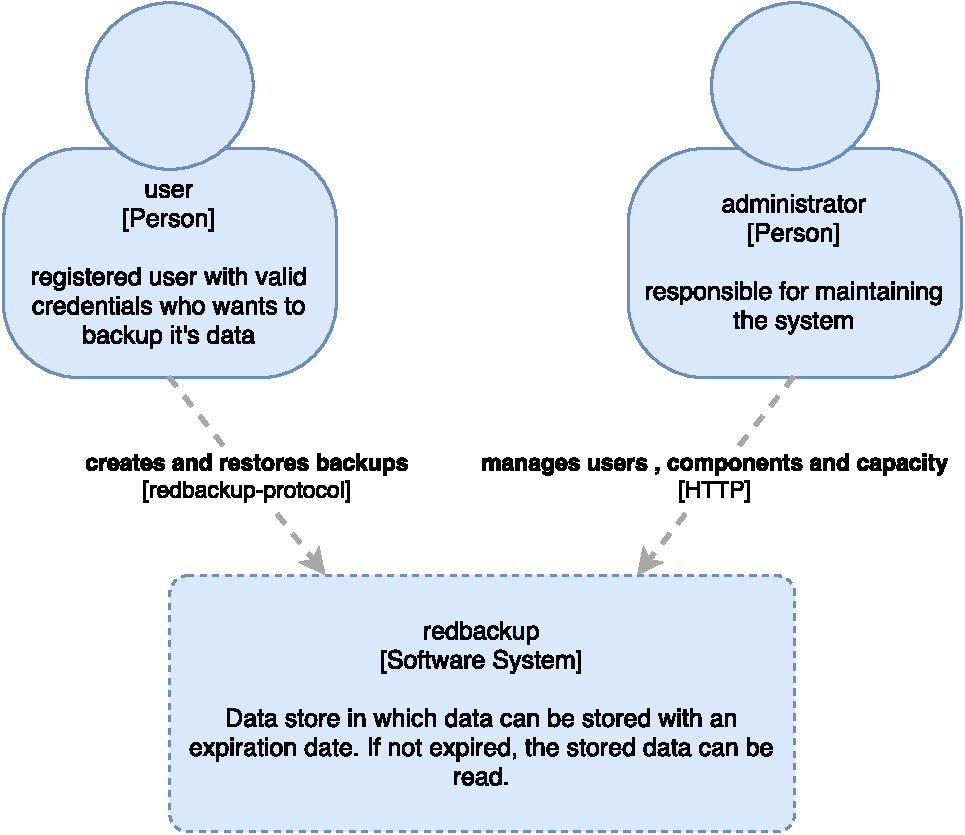
\includegraphics[width=0.8\linewidth]{resources/c4-overview}
	\caption[C4 System Context Diagram]{C4 System Context diagram showing the big picture.}
	\label{fig:c4-overview}
\end{figure}

Distinctive of both actors is that they do not want to interact directly with the system unless human interaction is inevitable. This takes the burden of manually creating backups away from the user including the risk of oblivion and minimises management efforts required by the administrator.  

Both actors, as well as their intentions, are described in more detail in Appendix \fullref{sec:specification}. Figure \ref{fig:c4-overview} presents a high-level overview that illustrates the interactions of the actors with the redbackup system.

\paragraph{Structure}
The redbackup system consists of four core components as shown in the C4 Container diagram in Figure \ref{fig:c4-container}.

\begin{figure}[h]
	\centering
	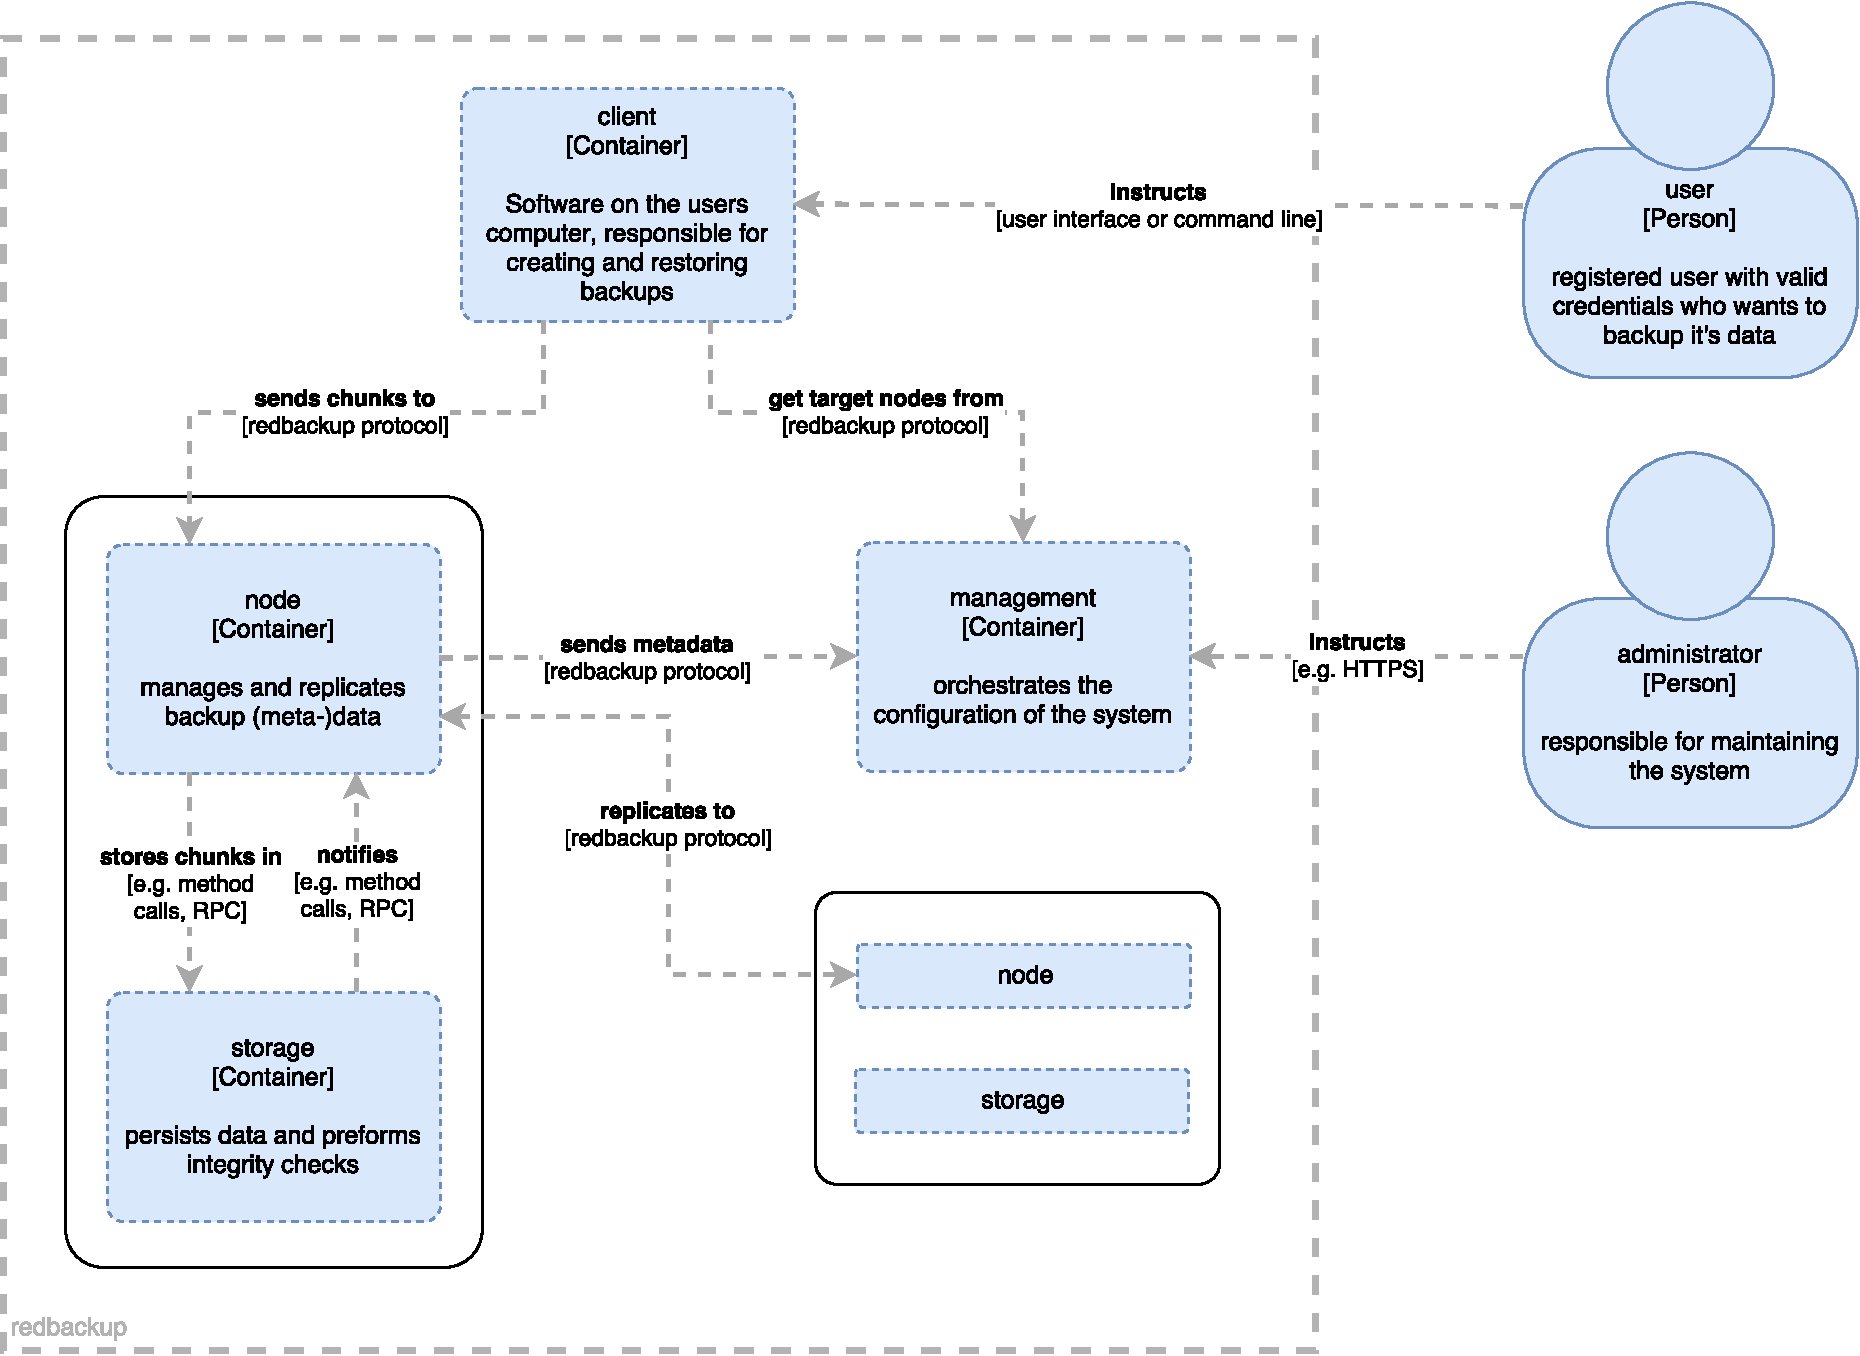
\includegraphics[width=1\linewidth]{resources/c4-container}
	\caption[C4 Container Diagram]{C4 Container diagram illustrating the high-level shape of the redbackup software system and how responsibilities are distributed.}
	\label{fig:c4-container}
\end{figure}

\paragraph{Client} A \gls{user} instructs a \gls{client} program typically running on the users machine to perform (unattended) backups and restores.  A \gls{client} persists and loads its data from one or more interconnected \glspl{node}.

\paragraph{Node}
A \gls{node} is in charge of data \glspl{chunk} including their replication onto other \glspl{node}. \Glspl{node} persist the actual data in a separate component, a \gls{storage}, to encapsulate persistence from replication and interaction to support different kinds of storage technologies (e.g. plain file systems or databases). A \gls{node} and its \gls{storage} are typically deployed on the same host.

\paragraph{Management}
One central \gls{management} component orchestrates the configuration of the system by providing metadata to \glspl{client} and \glspl{node}. This metadata includes user information and a set of all \glspl{node} in the system including their addresses and states. \Glspl{client} and \glspl{node} must cache this metadata which ensures that a temporary unavailability of the \gls{management} component does not compromise the replication and backup process.

All components including their responsibilities and interactions are described in more detail in Appendix \fullref{sec:specification}.

\paragraph{Protocols} Redbackup specifies a high-level protocol that is used for internal communication (noted in all C4 diagrams as \emph{redbackup protocol}). We deliberately specified the communication on a high level to encapsulate the underlying transport mechanisms.

\subsection{Backup creation}
\begin{figure}[h]
    \centering
    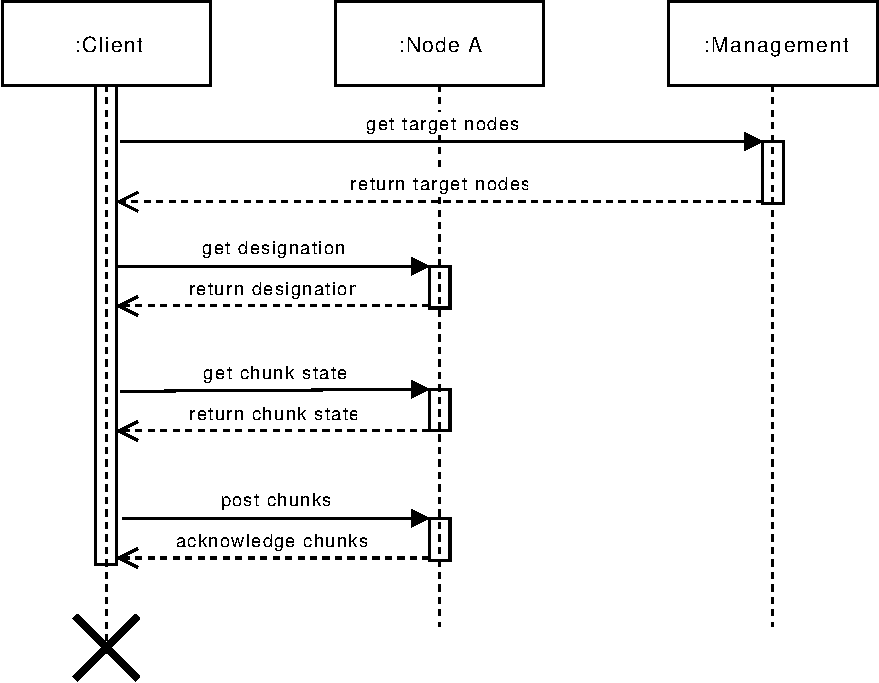
\includegraphics[width=\linewidth]{resources/create_backup}
    \caption{Create Backup UML Sequence Diagram}
\end{figure}

To create a backup, a \gls{client} loads \glspl{node}-metadata, that includes the addresses, from the \gls{management}. The \gls{client} caches this set and chooses one of them as \gls{designated-node}. This selection can either be random or based on heuristics, e.g. by analysing the round trip time to a \gls{node}.

The \gls{client} then requests permission to perform a backup on a given \gls{designated-node} by sending a \emph{get designation} message that includes an estimated backup size and the \gls{expiration-date}. If the \gls{designated-node} has the storage capacity as well as other resources available (i.e. it is not under overload), it confirms the designation request.

By now, the \gls{client} must start to build up backup metadata - hereafter called \gls{chunk-index} - by walking recursively through all directories to backup. Each file that is not explicitly excluded is split up into one or more data \glspl{chunk} using a rolling hash\cite{borg-data-structures}. Each of these \glspl{chunk} are then encrypted individually. Afterwards the \gls{client} derives the identifier of every \gls{chunk} based on its contents. This mechanism enables deduplication. Section \fullref{sec:fundamental-design-decisions} discusses \glspl{chunk} and \glspl{chunk-identifier} in detail.

The \gls{client} sends the calculated \glspl{chunk-identifier} at regular intervals to the \gls{designated-node}. The \gls{designated-node} returns a subset of all \glspl{chunk-identifier} of the \glspl{chunk} that are already present on it.

The \gls{client} then posts the missing \glspl{chunk} to the \gls{designated-node} which acknowledges successful receipt.

When all \glspl{chunk} are transmitted successfully, the client encrypts the \gls{chunk-index} as well and sends it to the \gls{designated-node} using the same mechanism as for any other \gls{chunk}. The only difference is that an additional flag - hereafter called \gls{root-handle} - is set so that it can be found again for restore.

The detailed backup scenario can be found in Appendix \fullref{sec:scenario-create-backup}.

\subsection{Backup restore}

\begin{figure}[h]
    \centering
    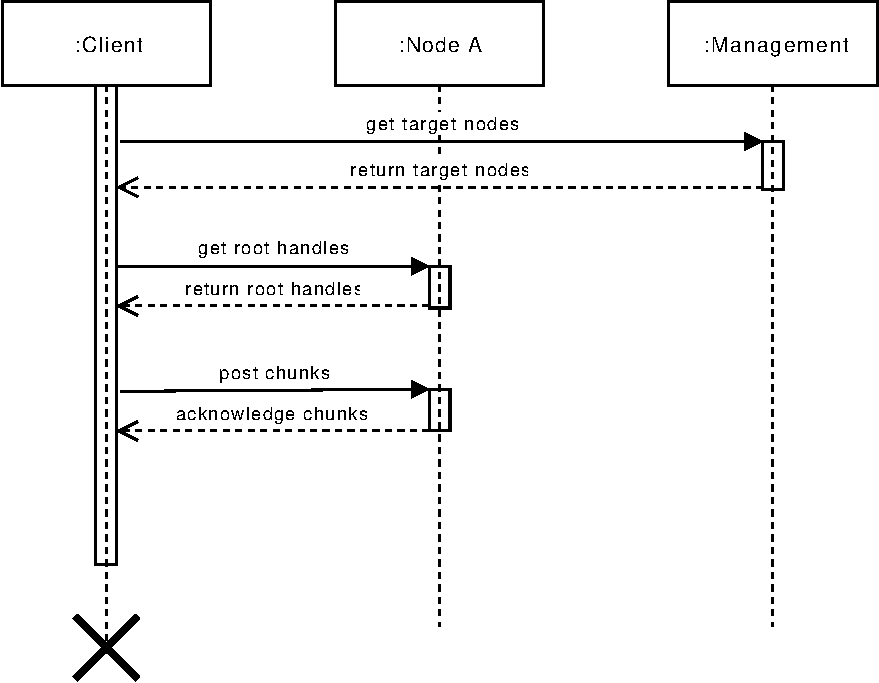
\includegraphics[width=\linewidth]{resources/backup_restore.pdf}
    \caption{Backup Restore UML Sequence Diagram}
\end{figure}

The restore mechanism works identical to the backup process up to the point where a \gls{designated-node} is chosen.

Next, the \gls{client} loads all \glspl{root-handle} from the \gls{designated-node}. The \gls{client} can decrypt the \glspl{chunk-table} from the returned \glspl{chunk-content}. Based on this information, the \gls{client} can provide multiple restore options to the \gls{user}, e.g. to restore a particular version of a given file.
With the user input and the previously fetched \glspl{chunk-table}, the \glspl{client} can calculate which \glspl{chunk} must be requested from the \gls{designated-node}. \Glspl{chunk-content} are then downloaded at regular intervals from the \gls{designated-node}, decrypted and combined.

\subsection{Replication}\label{sec:replication}
% Planned and unplanned leaving of nodes
% Management down
We deliberately only specified \gls{system-n-replication}, which means the degree of redundancy for the entire system is equal to the amount of \glspl{node} in the system (see \fullref{sec:fundamental-design-decisions}).

A \gls{node} is in charge of all data stored on it. Each \gls{node} - hereafter called \gls{sending-node} - randomly picks $n$ of its data \glspl{chunk}. It then picks one other \gls{node} randomly - hereafter called \gls{designated-node} - and requests which of the chosen data \glspl{chunk} remain persisted on the \gls{designated-node}. The \gls{designated-node} returns a subset of the requested \glspl{chunk} that consists of all \glspl{chunk} that it owns. Using this response, the \gls{sending-node} sends all missing \glspl{chunk} to the \gls{designated-node} which acknowledges successful receipt.

\begin{figure}[h]
    \centering
    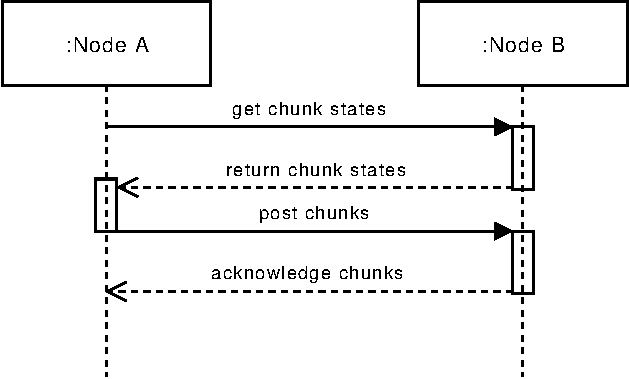
\includegraphics[width=0.6\linewidth]{resources/data_replication.pdf}
    \caption{Data Replication UML Sequence Diagram}
\end{figure}

This scenario is described in more detail in the Appendix \fullref{sec:scenario-data-replication}.

\subsection{Security and Encryption}\label{sec:security-and-encryption}
\paragraph{Data Integrity} One of our primary design goals is to ensure that once data is in the redbackup system, it cannot be altered or deleted from a \gls{client} to prevent ransomware attacks \cite{young-cryptovirology}. To achieve this, each backup is provided with an \gls{expiration-date} on which \glspl{node} are allowed to remove the associated data. 

Reasoning and potential risks of physical time are discussed in section \fullref{sec:removal-of-old-backups}.

\paragraph{Data Integrity on Nodes} Because \glspl{node} can also be the target of randsomware attacks, each \gls{node}, or more precisely its associated \gls{storage} component, must verify that given \glspl{chunk-content} are not corrupted. To be able to do so, it must be possible to calculate the identifier of such a data \gls{chunk} from its contents, using cryptographic hash functions.

A discussion on the role of hash functions including the chosen algorithms for the study project is carried out in section \fullref{sec:hash-collisions}.

\paragraph{Data Integrity on the Management} The \gls{management} component has no knowledge of the persisted data in the system. It only manages configuration and must not have detailed knowledge of \glspl{chunk} (need-to-know principle \cite{security-patterns}).

\paragraph{Data Encryption} A \gls{client} encrypts \glspl{chunk} when creating a new backup. This ensures that no other participant in the redbackup system can inspect file contents (need-to-know principle \cite{security-patterns}). The encryption and decryption keys are only stored on the \gls{client} and must be backed up separately.

\paragraph{Transport Security} All sent \glspl{message} should be signed by the sender. If so, transport layer encryption is not strictly necessary because all user data is already encrypted on the \gls{client} with the only exception of the \gls{expiration-date}.
\\
\vspace{1em}

\noindent A detailed description of these security mechanisms would be out of scope for this study project and will have to be carried out in a next step.

\subsection{Partitioning \& Scaling}

\paragraph{Availability \& Overload} To scale the redbackup system regarding availability, more \glspl{node} can be added to the redbackup system. If a given \gls{node} is overloaded, a \gls{client} can use another \gls{node} for backup creation or restore.

Because the backup and restore processes require approval of a \gls{designated-node} (see scenarios \fullref{sec:scenario-create-backup} and \fullref{sec:scenario-backup-restore}), an overloaded \gls{node} can finish work in progress backups/restores and reject new requests (following the patterns Finish Work In Progress and Shed Load \cite{fault-tolerance}). The data is replicated to overloaded \glspl{node} eventually.

We ensured that \glspl{node} are (mostly) stateless which simplifies scaling as well.

\paragraph{Storage Scalability} Because the proposed system currently only supports \gls{system-n-replication} (see section \fullref{sec:fundamental-design-decisions}), the maximum storage capacity is equal to that of the \gls{node} with the smallest storage. Therefore, to increase storage capacity, the capacity of all \glspl{node} must be extended to meet the desired amount.

To minimise network usage deduplication of data is used on the \gls{client}. Deduplication is  discussed in the paragraph Storage Unit in  \fullref{sec:fundamental-design-decisions}.

\subsection{Failure Detection}

Additionally to the above-discussed mechanisms for fault tolerance regarding security and scaling, the following failure detection mechanisms are in place.

\paragraph{Reporting} Most issues that occur on a \gls{node} are reported to the \gls{management} component (following the pattern Someone in Charge \cite{fault-tolerance}). The \gls{management} can then decide to notify the system administrator or execute error mitigation processes, e.g. suspend a given \gls{node} temporarily.

If a \gls{node} tries to connect to another \gls{node} that is not available, it notifies the \gls{management} component (following the pattern System Monitor\cite{fault-tolerance}).

Each \gls{node} periodically checks the persisted contents for possible corruption using the checksum mechanisms discussed in \fullref{sec:security-and-encryption} (following the Pattern Routine Audits \cite{fault-tolerance}). If a corruption is detected, the \gls{storage} notifies the \gls{node} which notifies the \gls{management}.

\paragraph{Single Point of Failure} For the case that the \gls{management} component is temporarily unavailable, \glspl{node} and \glspl{client} cache metadata, e.g. information about other \glspl{node}. Using these caches, \glspl{node} can perform replication and \glspl{client} manage their backups without interruption. Any notifications that were not successfully transmitted to the \gls{management} must be buffered on the \glspl{node} in order to ensure their delivery.

\section{Fundamental Design Decisions}\label{sec:fundamental-design-decisions}

We used the morphological box technique to explore different possible implementation options (see Table \ref{tbl:morphological-box}). The chosen option should be as simple as possible for the prototype developed in the study project but extensible for further adaption.

The following paragraphs reason the selected entry in each dimension.

\paragraph{Redundancy}

We originally planned to support \gls{client-m-replication}, which means that the \gls{client} defines a custom degree of redundancy from 1 to the number of \glspl{node} in the system. However, this is a complex mechanism that requires sophisticated algorithms to work correctly and efficiently. For the prototype, we chose the more straightforward implementation option system \gls{system-n-replication}, where the degree of redundancy for the entire system is equal to the number of \glspl{node} in it. Changing this option in the future will not be trivial because it requires additional changes in the replication process and the communication protocols.

\paragraph{Storage Unit}
The idea of \emph{chunks} come from Borg Backup. Files are partitioned into chunks using a rolling hash which enables deduplication and space efficient backups for large files \cite{borg-data-structures}. These are desired properties in a backup system to minimise network and disk usage.

\emph{Encrypting chunks} means that deduplication of the same file coming from different users is not possible anymore but is a necessity for privacy. Encryption is not trivial and requires a user concept that is out of scope of the prototype developed in the study project.
We chose the \emph{plain files} option for the study project to simplify the \gls{client} implementation. In the future, supporting \emph{encrypted chunks} will be possible by just modifying the \gls{client}.

\paragraph{Role of the Management}
The \emph{one in charge} option is the most straightforward option to implement, but conflicts with many intentions of the administrator (see \fullref{sec:adminstrator-intention}). We also intended to avoid a single point of failure. We chose the option \emph{autonomous replication} because it guarantees that replication is always ensured and keeps communication relatively simple.

\paragraph{Storage Backend}
Using the file system is the simplest possible solution for the study project and therefore the selected option. Adding support for other backends in the future is still possible because the storage component is an isolated part in the architecture (see \fullref{sec:component-storage}).

The number of files in a folder is limited depending on the used file system, length of a filename and other factors. Some file systems (e.g. ext4) have a global limit for the maximal number of files. This limit is 4 billion files for ext4. \cite{ext4}. Therefore we use the ext4 file system to persist data in the study project.

\paragraph{Removal of Old Backups}\label{sec:removal-of-old-backups}
We decided to use \emph{physical time}stamps that must be specified on backup creation. After expiration, the backup data may be removed by a garbage collector running on a \gls{node}. This may be extended to allow only mutual garbage removal in the future.

A significant problem that \emph{physical time} addresses is the safety of backup data in case a user computer is infected with malware~\cite{young-cryptovirology}. An illicit application might command the removal of backups or create new backups to initiate a garbage collection process to free storage capacity.

Nevertheless, the use of \emph{physical time} has the downside of possible data loss in case of wrong system times. To mitigate this risk, the system should use multiple distinct upstream time-servers. Multiple distinct upstream time-servers are used with a high probability as the proposed redundancy model motivates users to expand the system across multiple physical locations. Furthermore, the \gls{client}, \glspl{node} and \gls{management} should verify a reasonable accurate time when communicating mutually.

\paragraph{Programming Language \& Ecosystem}
We chose Rust over Erlang and Go because it offers great performance and minimal overhead supported by a powerful type system.
A complete language evaluation can be found in \fullref{sec:language-evaluation}.

\begin{sidewaystable}
	\centering
	\caption[Morphological Box]{Morphological Box}
	\label{tbl:morphological-box}
    \begin{tabu}{X | X X X X}
		\hline
          \textbf{Redundancy}
          & No redundancy
          & \Gls{client-m-replication}: The \gls{client} defines a custom degree of redundancy (from 1 to the number of \glspl{node}).
          & \Gls{system-m-replication}: The administrator defines the degree of redundancy for the entire system (from 1 to the number of \glspl{node}).
          & \textbf{\Gls{system-n-replication}}: The degree of redundancy for the entire system is equal to the amount of \glspl{node} in the system.
          \\ \hline

          \textbf{Storage unit}
          & \textbf{Plain files}
          & Encrypted files
          & Chunks: Cut files into multiple parts and store these individually.
          & Encrypted chunks: Same as chunks, but every chunk is individually encrypted.
          \\ \hline


          \textbf{Role of the management}
          & One in charge: The management knows and controls everything (e.g. the location of every file/chunk).
          & Configuration only: The management must be available for administrative tasks only. The \glspl{node} are mostly autonomous.
          & \textbf{Autonomous replication}: The management must be available for most of the tasks but replication also works if the management is down.
          & No management: Every \gls{node} is completely autonomous.
          \\ \hline


          \textbf{Storage backend}
          & \textbf{Plain filesystem}: Store all files/chunks as files in one directory with a unique identifier.
          & Database: Use an existing database solution (e.g. Git, Redis, RocksDB).
          & Cloud Storage: A proxy to a cloud storage provider (e.g. Amazon S3).
          & Custom: An optimized version of the plain file system option with optimised indexing and compression.
          \\ \hline


          \textbf{Removal of old backups}
          & \textbf{Physical time}: Data is removed on a specified physical time.
          & User command: The user commands removal of data.
          & Free storage: Data is removed, as soon as capacity issues occur.
          & Physical time with mutual agreement: All \glspl{node} must agree before data is removed.
          \\ \hline


          \textbf{Programming language / ecosystem}
          & \textbf{Rust}
          & Go
          & Erlang
          & 
          \\ \hline
	\end{tabu}
\end{sidewaystable}

\subsection{Hash Collisions}\label{sec:hash-collisions}
To achieve deduplication and space-efficient backups for large files, as discussed above, a chunk identifier must be derived from the actual chunk contents. 
A common mechanism used to derive identifiers from binary data is the use of cryptographic hash functions. Most cryptographic hash functions produce a message digest that has a fixed length (e.g. SHA-256\cite{sha-256} produces a 256-bit digest) for a given message with an arbitrary length. The restricted lenght can theoretically lead to collisions.
Perfect hash functions do not have this property because their input message lenght is equal to the lenght of the resulting message digest. A perfect hash function is not practical in our case due to the large message digests.
With cryptographic hash functions, collisions are possible but unlikely. Assuming that the applied function does produce equally distributed results, the probability can be calculated based on the birthday problem\cite{birthday-attack} as follows, where $p$ is the number of chunks in the system and $n$ the lenght of the message digests:

\[
P(p, n) = \frac{p^2}{2^{n+1}}
\]

Assuming we have $p=30^{21}$ chunks the system (which is equivalent to two billion years of music assuming each chunk has a size of one byte\cite{seagate-zetabyte}) and using the SHA-256 algorithm, the probability of a collision is about $4.72 \cdot 10^{-16}$, which is highly improbable and may therefore be neglected.

However, did a collision occur after all, for example, if the used cryptographic hash function were flawed or the unlikely event occured, it would result in data loss.

In theory, we could detect collisions on the \gls{client}. To do so, every time an identifier is calculated, the \gls{client} must verify that if a chunk with the same identifier already exists in the system, it has the exact same contents. If the contents differ, it is a collision. This approach requires a lot of network traffic and can slow down the backup process significantly.

Another place to detect collisions is on the \gls{node} component. A \gls{node} can verify if the contents of a given chunk are equal to the contents already present in the system. The downside of this approach is that it requires the \gls{client} always to send the full contents of every chunk, which leads to a lot of additional network traffic.

Both of the described approaches for collision detection have significant costs that are not practical.

As for the study project, we use the SHA-256 algorithm\cite{sha-256} and neglect the risk of hash collisions due to its low probability. Nonetheless, we prepare all protocols and components to use an interchangeable mechanism for the calculation and transmission of file/chunk identifiers.

\section{Prototype}\label{sec:prototype}

Because the entire system, as described in the previous sections, is too large and complex to implement in the form of a study project prototype, we reduced the functionality to its core.

Our prototype focuses on the backup, restore and replication scenarios as described in Appendix \fullref{sec:scenarios} leaving out encryption.

We also limited the supported platforms to 64-Linux only as this is the operating system we use for development and continous integration.

The implemented prototype is organised in 46 modules, defines 188 functions and has 4'240 lines of code, including unit test code and whitespace. All components are implemented using the Rust programming language \cite{rustlang-org}. Installation instructions are documented in the project's repository.

\subsection{Concrete Architecture}

Figure \ref{fig:c4-sa-container} illustrates the system as implemented in our prototype.

\begin{figure}[h]
	\centering
	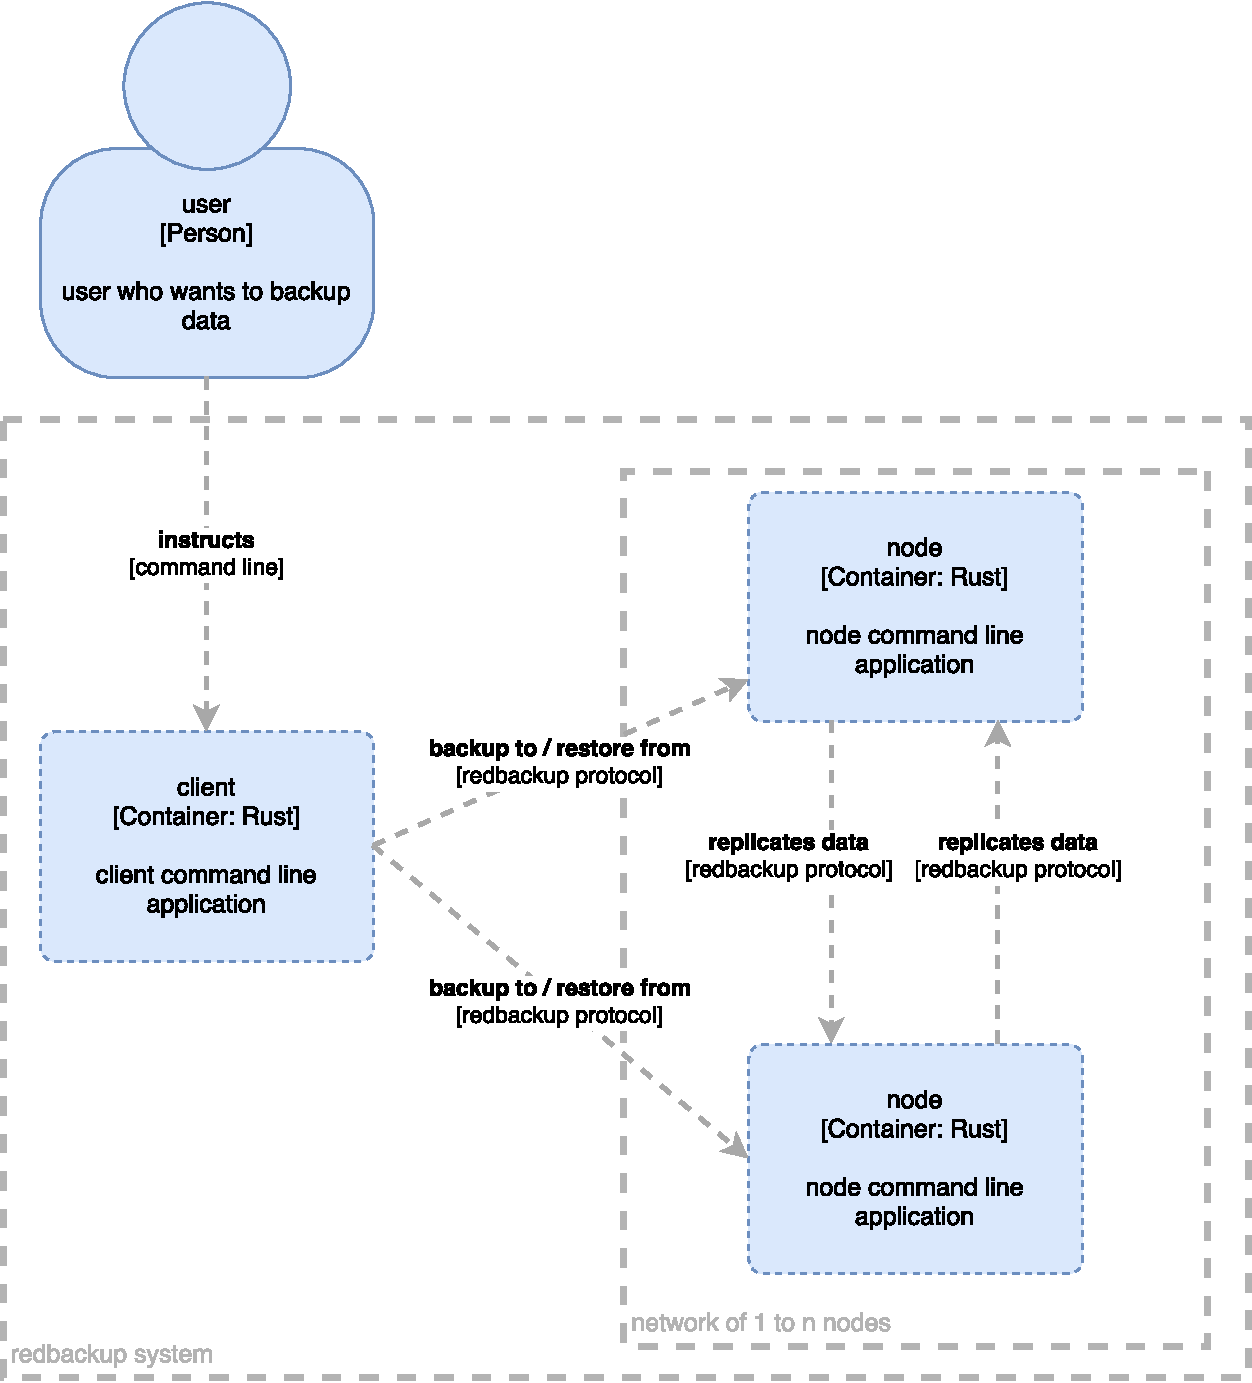
\includegraphics[width=0.8\linewidth]{resources/c4-sa-container}
	\caption[Study Project specific C4 Container Diagram]{C4 Container diagram illustrating the high-level shape of the prototype and how responsibilities are distributed as implemented in the study project.}
	\label{fig:c4-sa-container}
\end{figure}

The \gls{client} and \gls{node} are delivered as executables that are configured and launched using the command line.

The \gls{node} component binds itself to a configured network interface and port on which it provides the services for backup creation, backup restore and replication.

The \gls{client} executable is started individually for every operation that is the creation of a backup, listing all backups persisted on a given \gls{node} and data restore.

\subsubsection{Client}

The \gls{client} executable bundles three components as shown in Figure \ref{fig:c4-client-container}.

\begin{figure}[h]
	\centering
	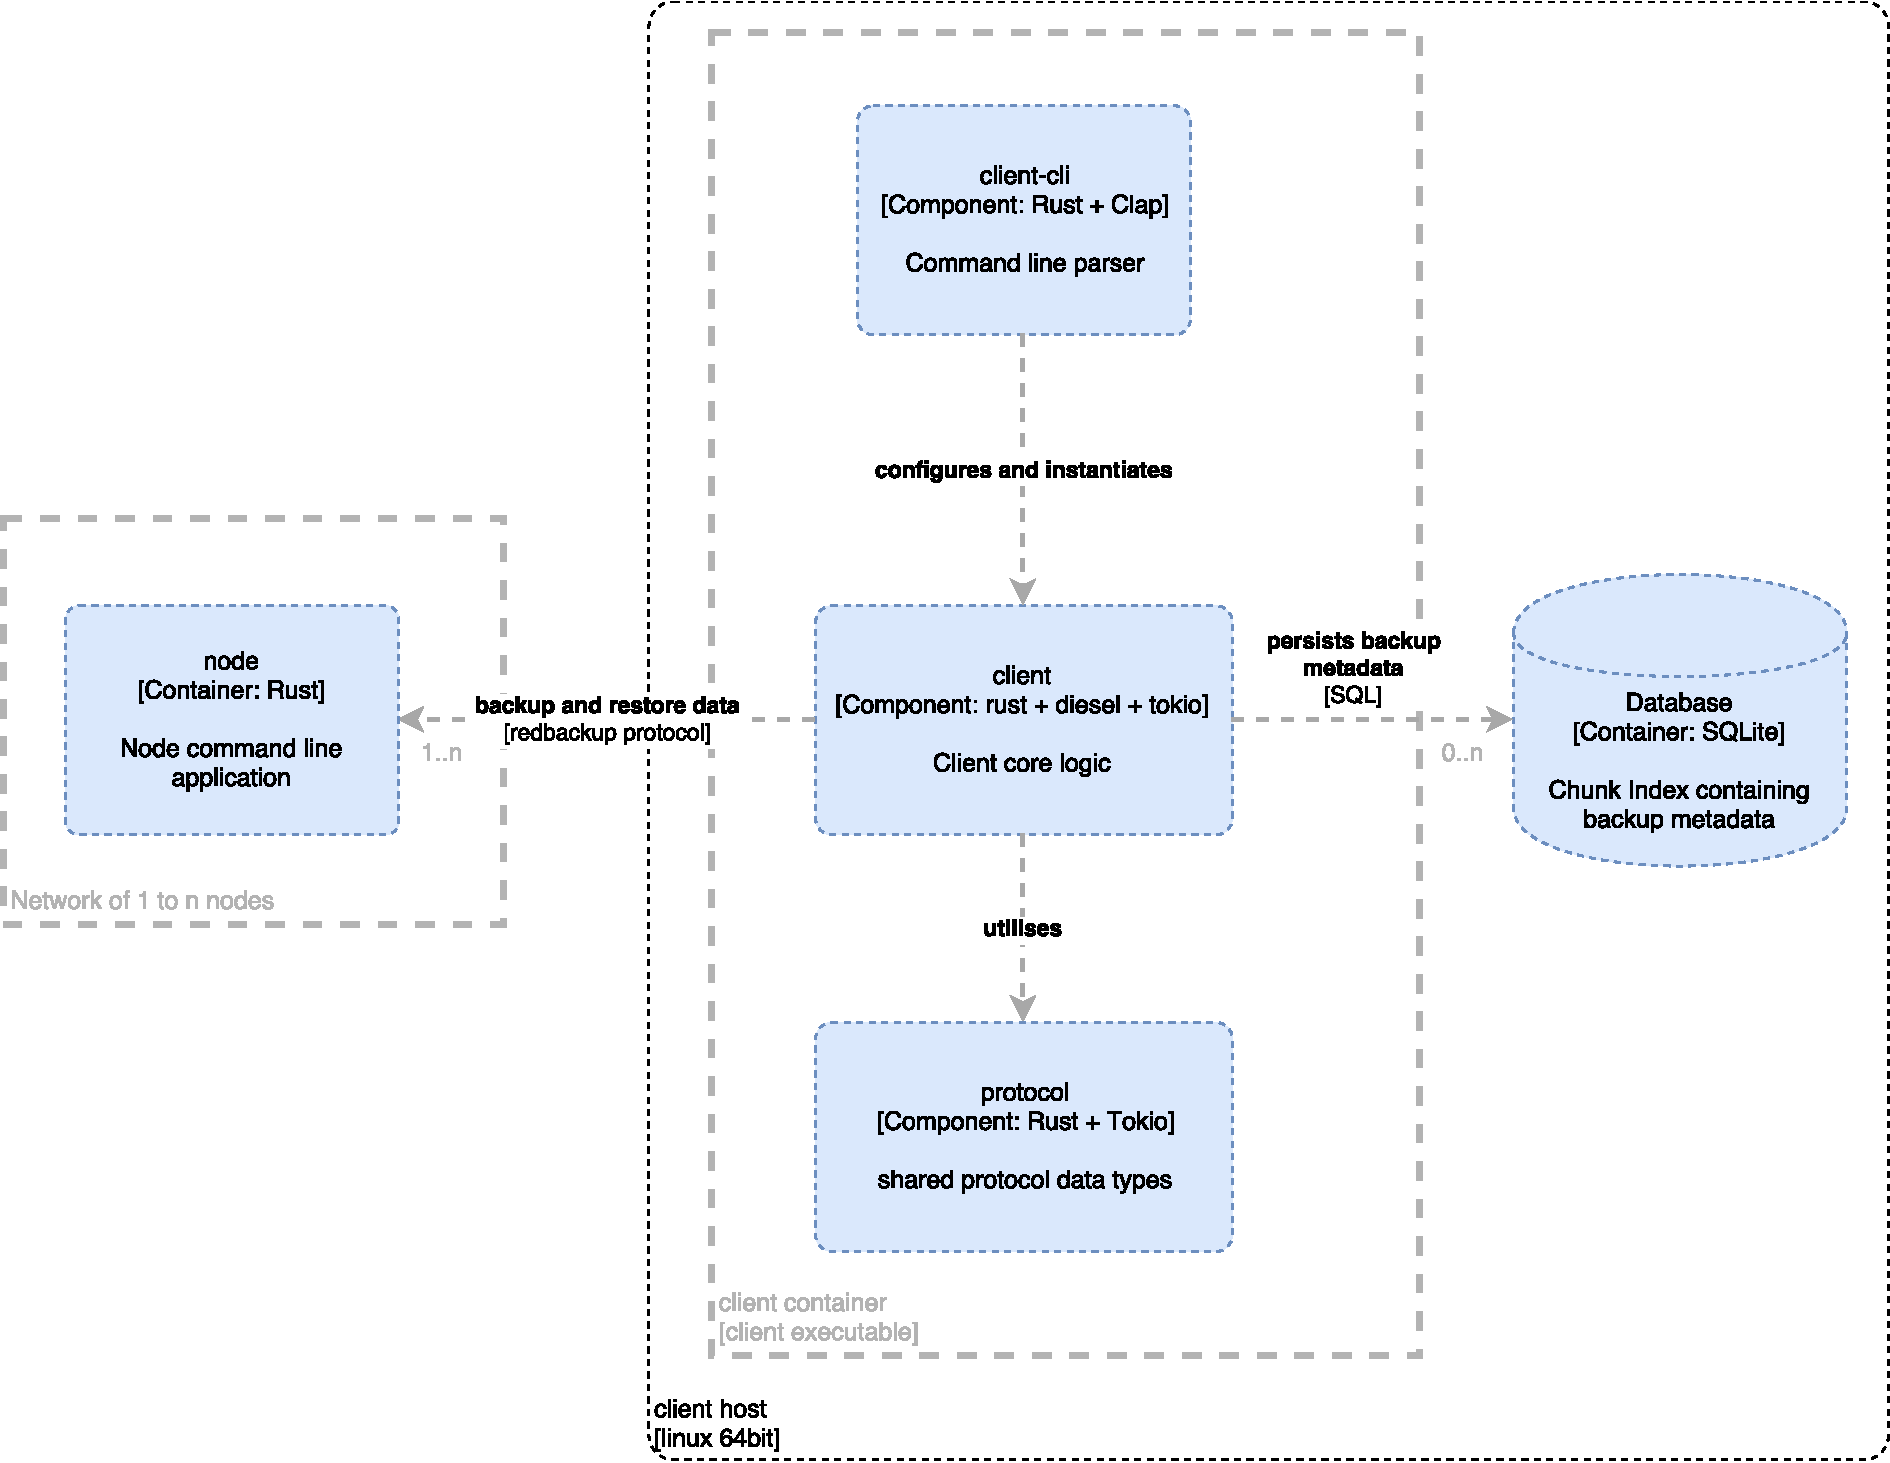
\includegraphics[width=1\linewidth]{resources/c4-client-container}
	\caption[Client specific C4 Container diagram]{C4 Container diagram illustrating the shape of the \gls{client} and how responsibilities are distributed as implemented in the study project.}
	\label{fig:c4-client-container}
\end{figure}

\emph{Client-cli} contains the command line specific logic that provides an uncluttered interface for advanced users and serves as an entry point in the client's core logic. We used the clap\footnote{\url{https://clap.rs/}} library to implement this component. The command line interface is described in Appendix~\ref{sec:prototype-command-line-interface}.

The \emph{client} component contains the actual logic for creating and restoring backups. It is organised as a library so that it can be used from other projects as well, e.g. if we provide a graphical user interface in the future. The \gls{client} component creates the \gls{chunk-index} for every backup in a separate \emph{SQlite-database}. For database access, we used the Diesel\footnote{\url{https://diesel.rs/}} ORM-library.

The \gls{client} components make heavy use of a networking library called tokio\cite{tokio-rs} that provides an efficient event loop similar to the Reactor pattern \cite{POSA1}. Although tokio supports highly parallel networking code, we decided to implement all interactions on the \gls{client} serial to maintain readability.

The (de-) serialisation mechanisms for messages sent to and received from \glspl{node} are encapsulated in the \emph{protocol} component, following the Forwarder Receiver Pattern \cite{POSA1}.

We opted for Diesel and tokio because there are currently no comparable alternatives on the marked for both.

In the prototype, the \gls{client} interacts with one \gls{node} at a time to maintain simplicity. The \gls{node} to interact with is passed to the \gls{client} executable via command line arguments.

\subsubsection{Node}

The \gls{node} executable bundles four components as shown in Figure \ref{fig:c4-node-container}.  

\begin{figure}[h]
	\centering
	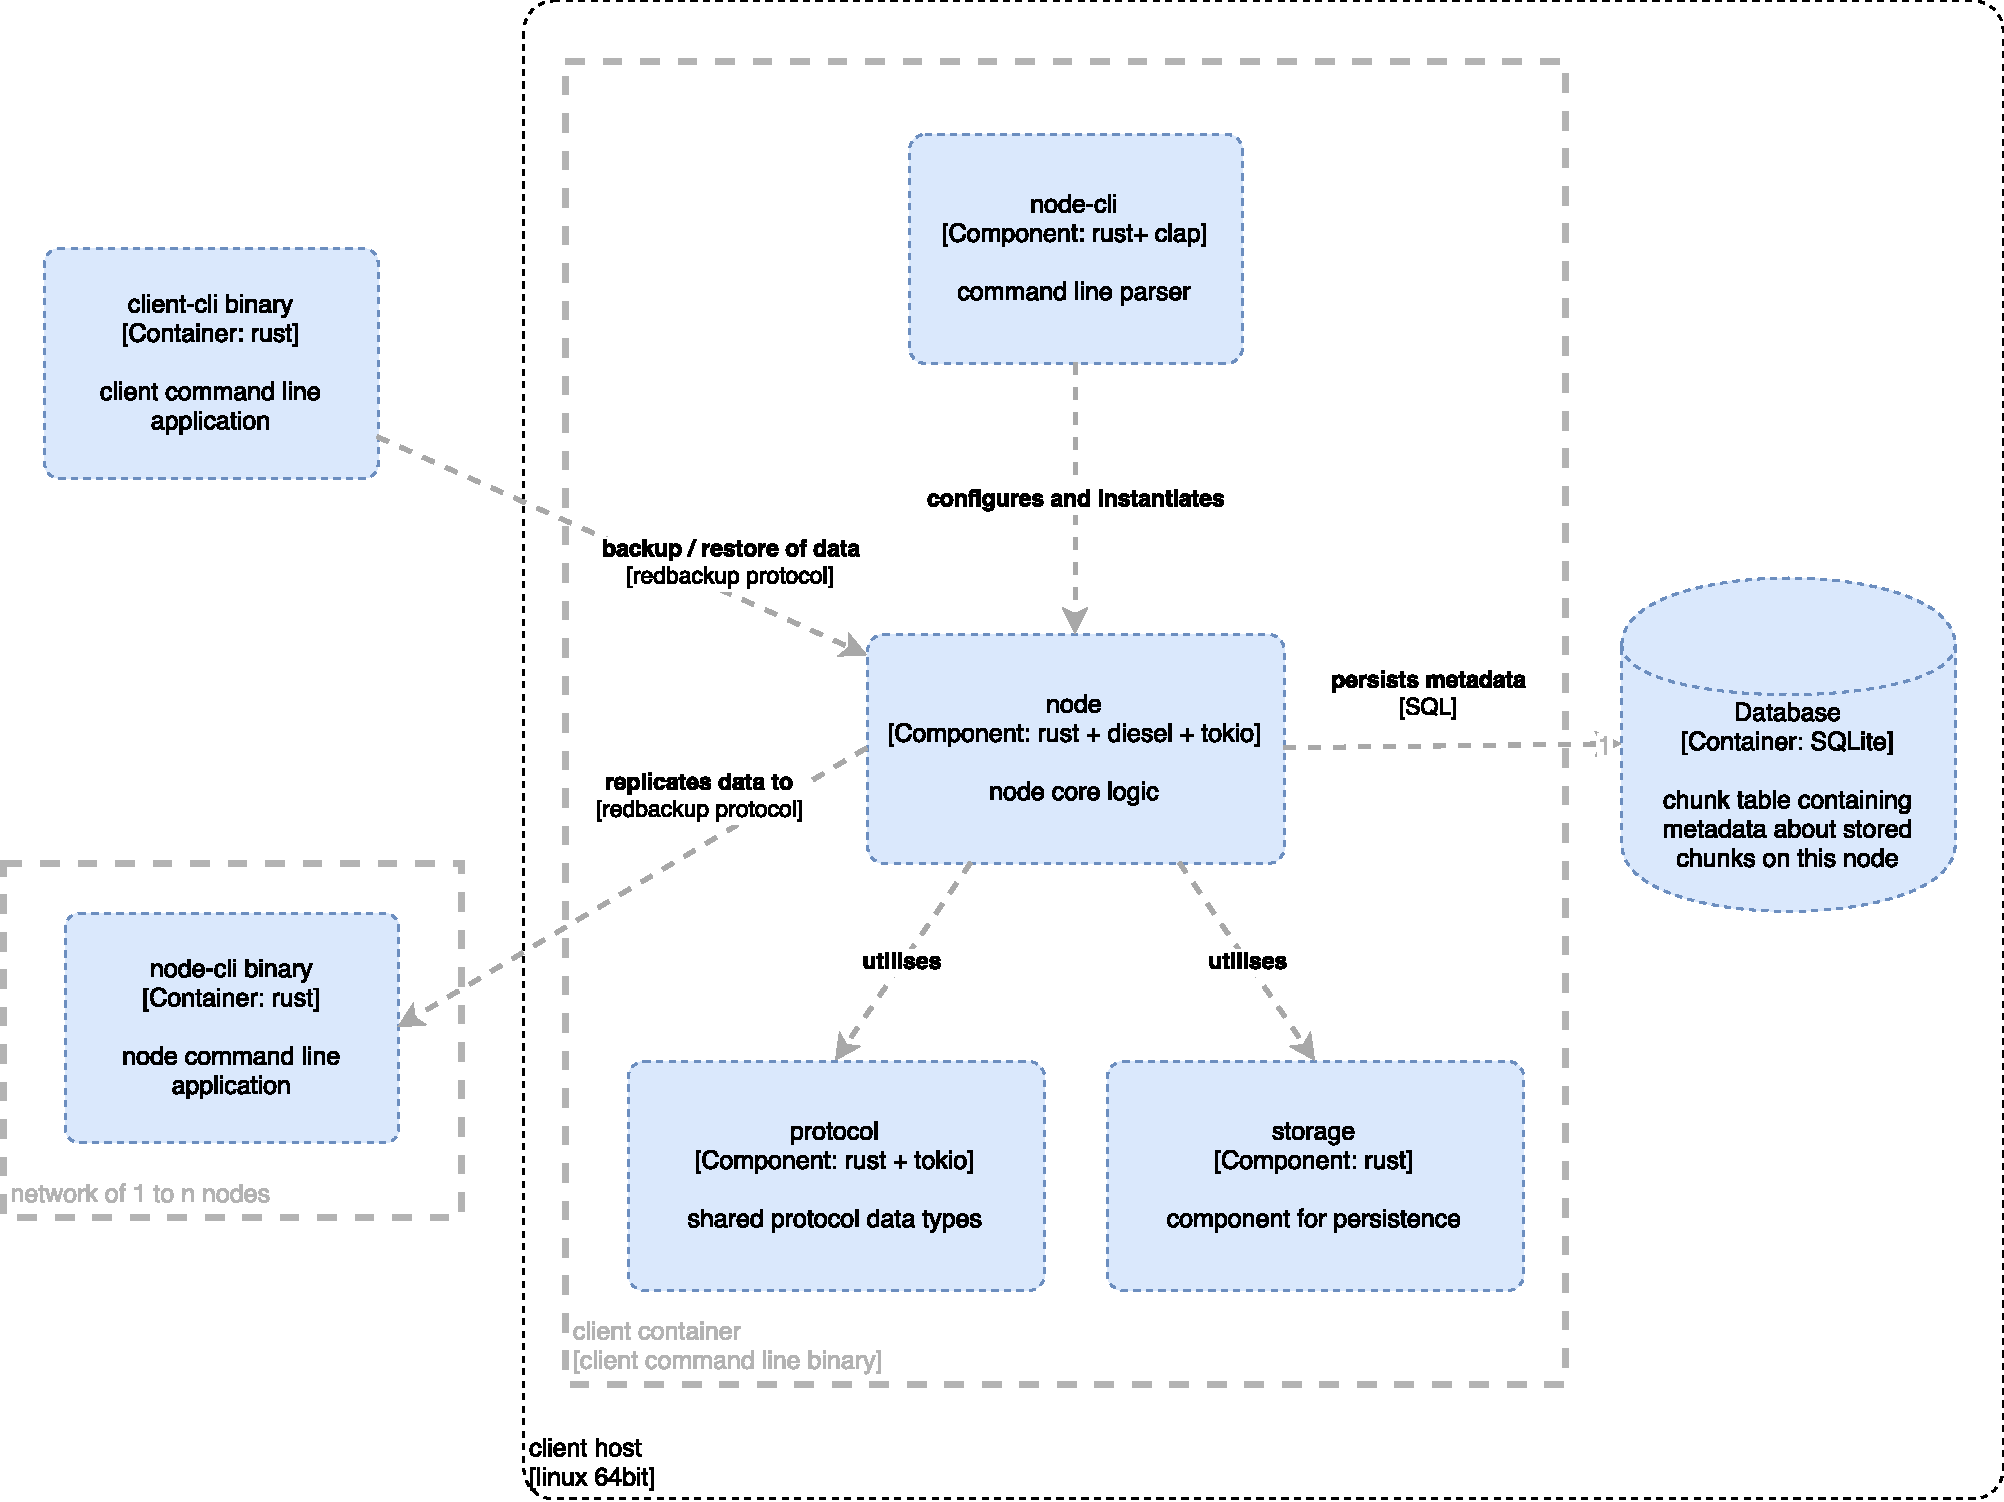
\includegraphics[width=1\linewidth]{resources/c4-node-container}
	\caption[Node specific C4 Container diagram]{C4 Container diagram illustrating the shape of the \gls{node} and how responsibilities are distributed as implemented in the study project.}
	\label{fig:c4-node-container}
\end{figure}

Just like the \gls{client} implementation, the command line logic is encapsulated in a separate component called \emph{node-cli}.

The core logic is implemented in the \emph{node} library. Like the \gls{client}, the \gls{node} component makes heavy use of the tokio and Diesel libraries. In contrast to the client, we used the parallel features of tokio. To keep the chosen technology close to the client, we decided to use SQLite for the \gls{chunk-table}. This must be changed in the future because SQLite locks the entire database when writing, which makes concurrent updates impossible \cite{sqlite-locking}.

We use the same \emph{protocol} component for (de-) serialisation of messages on the \gls{node} and the \gls{client}.

The \emph{storage} component is also bundled directly in the \gls{node} executable. It persists data in one single directory as described in \fullref{sec:fundamental-design-decisions}.

Other known \glspl{node} are passed to the \gls{node} executable via command line arguments.

Because user authentication requires additional cryptographic efforts, the prototype accepts backups and replications from everyone.

\subsection{Testing}\label{testing}

In the following subsections, we describe how the prototype and architecture can be tested.

\subsubsection{Unit Tests}\label{unit-tests}
Test Driven Development (TDD) \cite{TDD} should be used as much as possible. Our Definition of Done (Appendix \ref{sec:project-plan}) states that \emph{reasonable unit and integration tests [must] exist and pass.}

All unit tests are executed on every build run on our continuous integration server. That is on every repository push and pull request.

\subsubsection{Integration Tests}\label{integration-tests}

We defined two primary environments for the integration tests: A minimal network as defined in Figure \ref{fig:integrationtestsmall} and a medium one, as defined in Figure \ref{fig:integrationtestmedium}.

\begin{figure}
	\centering
	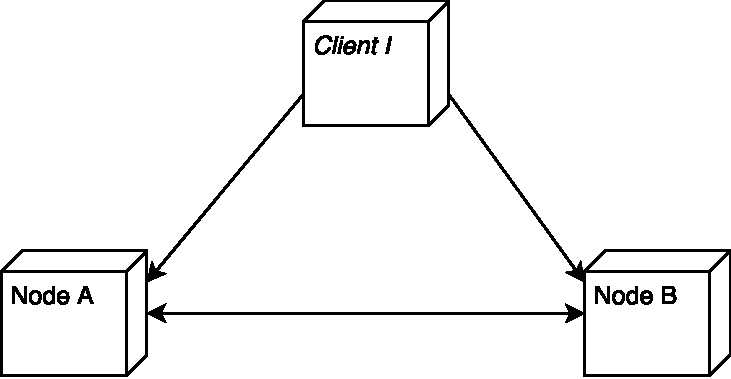
\includegraphics[width=0.5\linewidth]{resources/integration_test_small}
	\caption[Minimal integration test]{Minimal integration test with one \gls{client} and two \glspl{node}.}
	\label{fig:integrationtestsmall}
\end{figure}

\begin{figure}
	\centering
	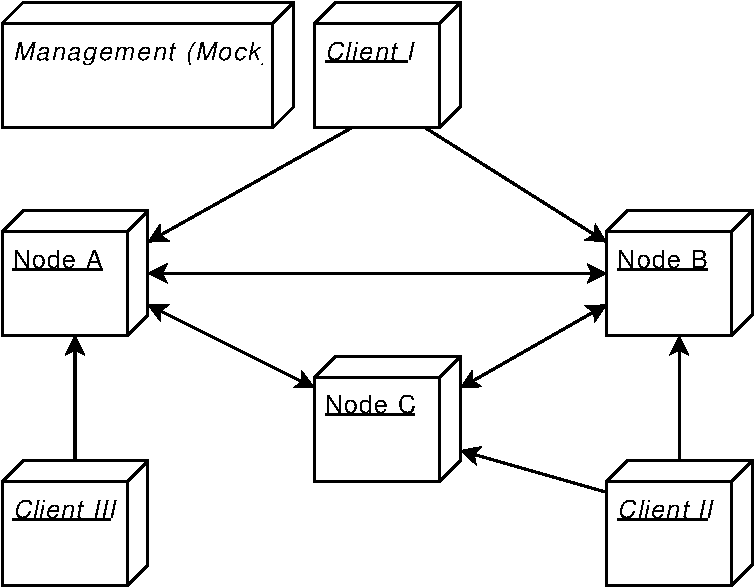
\includegraphics[width=0.5\linewidth]{resources/integration_test_medium}
	\caption[Medium integration test]{Medium integration test with three \glspl{client} and three \glspl{node}.}
	\label{fig:integrationtestmedium}
\end{figure}

These two rather small network styles will most commonly be deployed, yet they can produce most of the possible problems.

The integration tests are run automatically at least on every tagged release (i.e. at least once every sprint). Because of the (yet) well managable set of integration tests for the prototype, these tests can run on every build as well.

Tests for fault tolerance, e.g. what happens if a \gls{node} goes down while receiving data, can be implemented as integration tests as well.

\subsubsection{Architecture tests}

Architectural tests are special and manually run tests to verify the scalability of our software architecture.